\documentclass{boi2014}

\usepackage{enumitem}

\renewcommand{\DayNum}{2}
\renewcommand{\TaskCode}{senior}
\renewcommand{\TaskName}{Senior Postmen}

\begin{document}

    It is the year 2036 and Europe is crowded by senior citizens. In order to
    keep them healthy, the European ministry for majority groups (seniors
    \emph{are} a majority!) suggests to have them deliver the small amount of
    paper mail that is still being sent --- typically to seniors. This
    suggestion is going to be implemented all over Europe, even in the Free
    States of Norway and Switzerland.

    The ministry has devised a "senior postmen system" in the following way:
    Europe has been divided into mail districts. A mail district has a street
    network of streets and junctions. Every street in the network can be walked
    in both directions. In each district, arbitrarily many senior citizens are
    available to be hired as mailman. Every morning, each mailman receives a bag
    with mail to be delivered on a tour that covers a part of the street
    network. Every tour must be senior--compatible, i.~e. it must satisfy the
    following conditions:

    \begin{itemize}
        \item It starts and ends at the same junction. (Hey, it’s a tour!)
        \item It never passes a junction more than once. (The seniors shall not
        be confused.)
        \item It must not have a street in common with any other tour; hence,
        any street in the district is to be served by exactly one mailman. (The
        seniors shall not fight with each other.)
    \end{itemize}

    Together, the tours must cover the given network: each street in the network
    must be part of exactly one tour.

    \Task
    The ministry now needs a software that, for a given mail district’s street
    network, will compute a set of senior--compatible tours that cover the
    network.

    \Input
    The input describes the street network.

    The first input line contains two integers $N$ and $M$. $N$ is the number of
    junctions, and $M$ is the number of streets. Junctions are numbered from 1
    to $N$.

    Each of the following $M$ lines contains two integers $U$, meaning that
    there is a street connecting junctions $U$ and $V$.

    For any input holds:
    \begin{enumerate}
        \item For any two junctions, you can walk from one junction to the other.
        \item There is a solution, i.e. a set of senior-compatible tours can be
        computed that cover the network.
    \end{enumerate}

    \Output
    The first output line is to contain an integer $T$, the number of tours.

    The $T$ tours are described in the following $T$ lines. Each of these lines
    is to contain at first the number $C$ of different junctions the mailman has
    to pass on this tour. The following $C$ integers in the line are the numbers
    of the junctions in this tour. They must be output in the order the
    junctions are passed by the mailman, with the starting (and ending) junction
    being output first (and only once).

    If there are two or more solutions, your program may output any of them.

    \Example

    \example
    {
        10 15 \newline
        1 2 \newline
        5 1\newline
        2 3 \newline
        9 2\newline
        3 4 \newline
        6 3\newline
        4 5 \newline
        7 4\newline
        4 8 \newline
        5 7 \newline
        8 5\newline
        6 7 \newline
        7 8 \newline
        8 10 \newline
        10 9
    }
    {
        3 \newline
        7 2 3 4 5 8 10 9 \newline
        3 4 7 8 \newline
        5 1 5 7 6 3
    }
    {
        The following picture illustrates the street network and the three
        senior-compatible tours that may be used to cover it.

        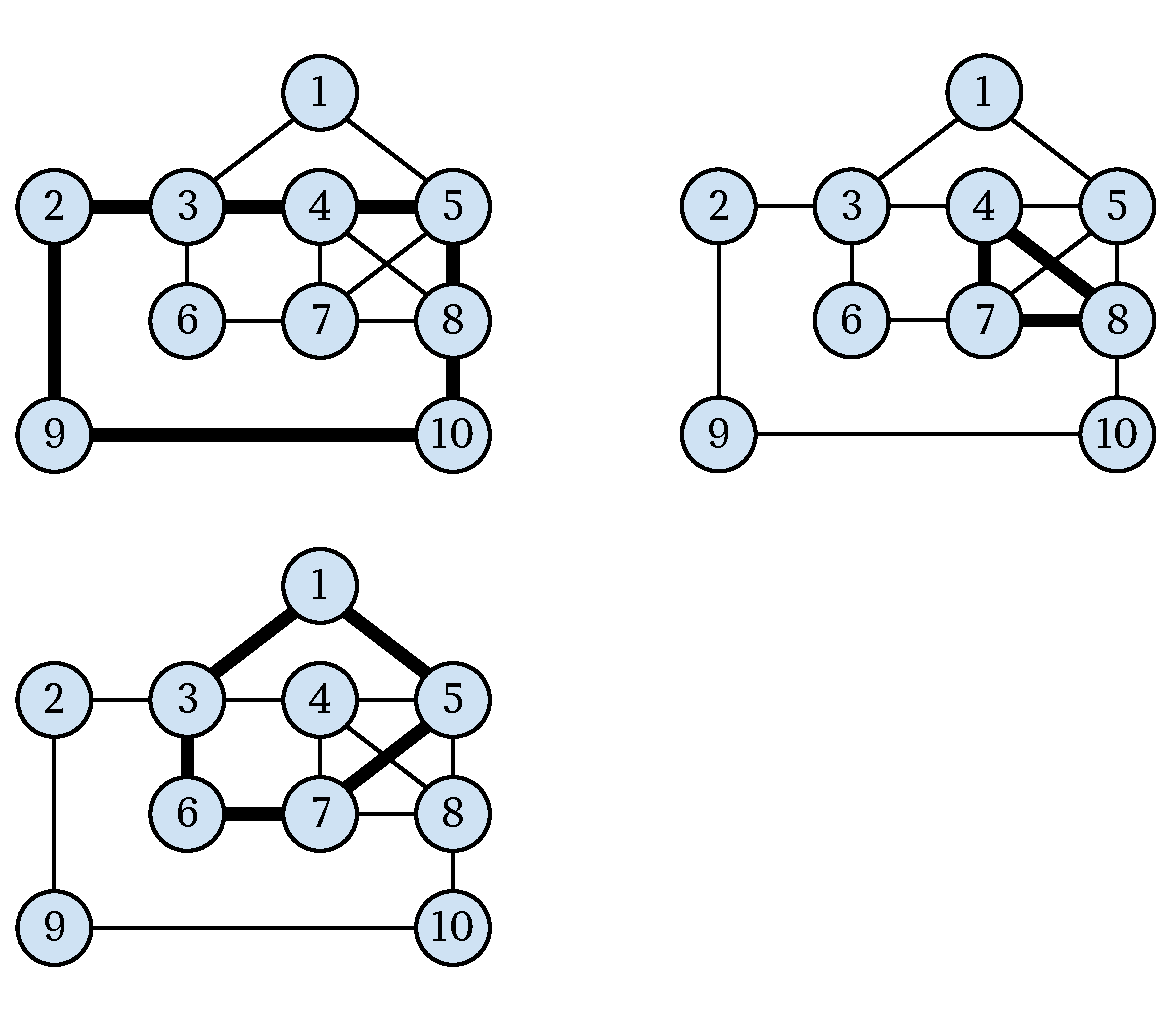
\includegraphics[width=7cm]{senior-example}

        Note that there are several solutions to this example, among them some
        with only two tours.
    
    }

    \Scoring

    \begin{description}
        \item[Subtask 1 (40 points):] $1 \le N \le 2\ 000$, $1 \le M \le 100\ 000$.
        \item[Subtask 2 (20 points):] $1 \le N \le 100\ 000$, $1 \le M \le 100\ 000$.
        \item[Subtask 3 (40 points):] $1 \le N \le 1\ 000\ 000$, $1 \le M \le 1\ 000\ 000$.
    \end{description}

    \Constraints

    \begin{description}
        \item[Time limit:] 2 s.
        \item[Memory limit:] 256 MB.
    \end{description}

\end{document}
